\section{Theory}
\label{sec:Theory}

\subsection{Basics of Lasers}
\label{ssec:laser_basics}

A laser is a source of electromagnetic radiation such as visible light that has properties conventional light sources such as a light bulb cannot fulfill simultanously.
The most important of these properties of the emitted radiation are: 
\begin{itemize}
    \item high intensity
    \item low divergence, i.e. highly focused
    \item narrow bandwidth, i.e. monochromatic
    \item high coherence length
\end{itemize}

Because of those properties lasers are widely used nowadays. 
Use cases can be laserpointers, lightshows, distance measurements, lasercutters, data storage via optical drives, laserprinters, fiber-optics and many more.
One of those use cases is spectroscopy and this is what we will do in this experiment.

Laser is the abbreviation for "light amplification by stimulated emission of radiation".
Therefore a laser operates in such a way that energy is pumped into a medium so that the atoms can be excited.
If enough atoms are excited (i.e. population inversion) a single photon can stimulate an atom such that it emits another photon.
The so produced radiation is reflected back and forth in some kind of resonator where it can stimulate more emissions.
A certain ratio of photons can escape the resonator and those photons now have the previously mentioned properties.

The classical technology for lasers are dye lasers, but those lasers are expensive and difficult to use.
The use of semiconductor laser diodes have changed this drastically.

\subsection{Basics of Diode Lasers}
\label{ssec:diode_laser_basics}

\begin{figure}
    \centering
    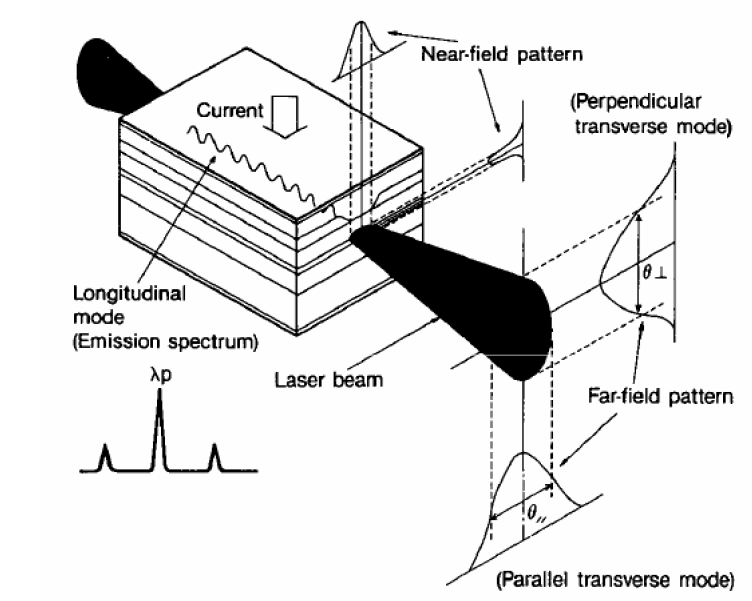
\includegraphics[width=0.5\textwidth]{images/laser_diode_scheme.png}
    \caption{Schematic view of a laser diode chip \cite{V60}}
    \label{fig:laser_diode_scheme}
\end{figure}

A diode laser is constructed of a minimum of three layers, the n-layer, the active layer and the p-layer.
A basic scheme of a diode laser can be seen in \autoref{fig:laser_diode_scheme}.
The n- and p-layers are doped so that they are charged negative (electrons) or positive (electron holes).

When injection current is run through the diode the active layer is injected with both the electrons and electron holes.
The process of recombination emits a photon. 
Another photon can cause this emission to be stimulated.
The amount of amplification by stimulated emission is called the optical gain.
The surfaces of the n- and p-layers are made highly reflective so that the active layer is an inner cavity for the photons and inside is a standing wave.

The emitted radiation can escape the inner cavity at the front facet or the back facet.
Although the laser diode used in this experiment has a coated back facet so that most of the radiation is reflected back.

A laser diode only starts to lase above a certain threshold current. 
Below this threshold it operates more like a LED.
Above the threshold the radiation is coherent and the intensity increases linearly with the injection current.
It should be noted that the emitted radiation is highly divergent and has a large bandwidth compared to the bandwidth of atomic transitions.

\begin{figure}
    \centering
    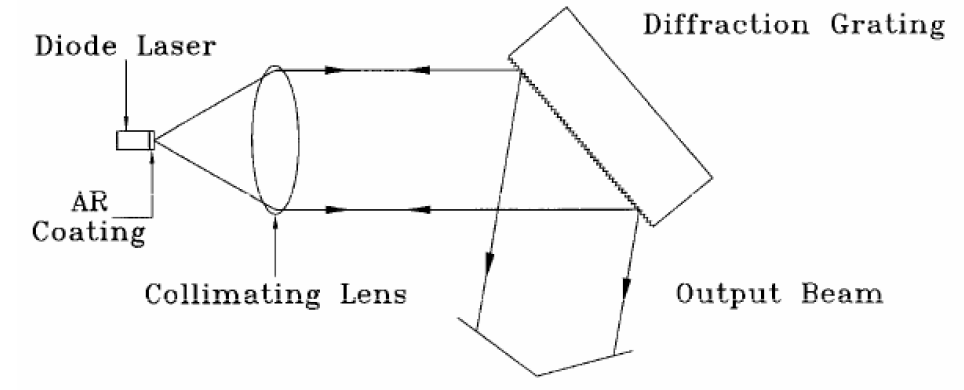
\includegraphics[width=0.7\textwidth]{images/grating_feedback_scheme.png}
    \caption{Schmeatic configuration of a laser diode using grating feedback \cite{V60}}
    \label{fig:grating_feedback_scheme}
\end{figure}

A configuration like shown in \autoref{fig:grating_feedback_scheme} is used to solve multiple problems a bare laser diode has.
The lense collimates the highly diverging radiation into a beam.
The optical grating is used to feed a small portion of the emitted radiation back into the laser diode but prevent external radiation to enter the laser diode.
This creates an external cavity and helps with stabilizing and narrowing the frequencies of the emitted radiation.
With this a bandwidth can be achieved that is much smaller than the bandwidth of atomic transitions.


\subsection{Tuning a Diode Laser}
\label{ssec:laser_tuning}

Once the laser is lasing it emits mostly radiation of a single frequency.
While this frequency depends on many different factors, it is just the frequency where the net optical gain is the highest.

\begin{figure}
    \centering
    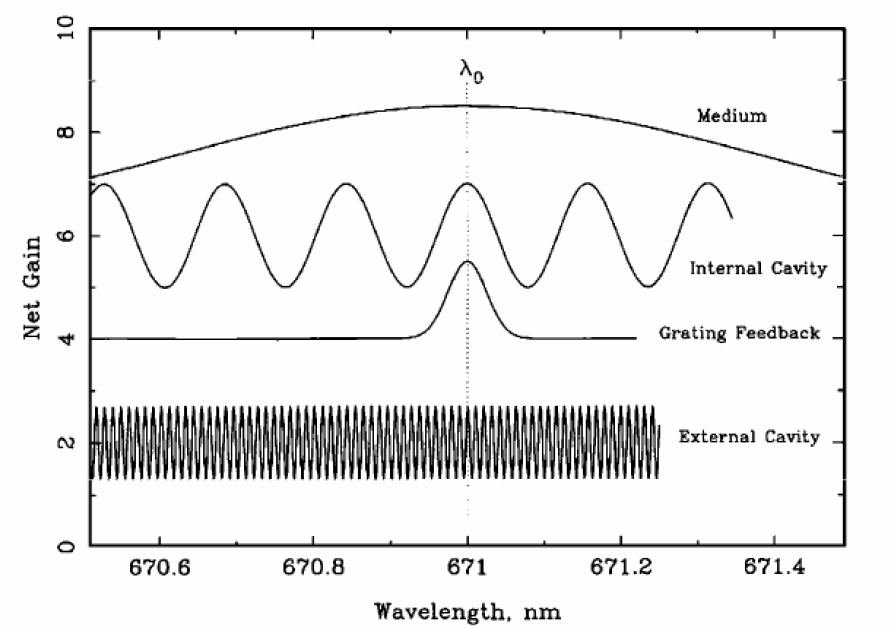
\includegraphics[width=0.8\textwidth]{images/frequency_contributions.png}
    \caption{Schematic of the different contributions to the net optical gain of an arbitrary laser as a
    function of frequency. The curves are displaced relative to one another for clarity. \cite{V60}}
    \label{fig:frequency_contributions}
\end{figure}

In \autoref{fig:frequency_contributions} you can see the different contributions to the laser frequency.
Those contributions will be discussed in the following sections.

\subsubsection{medium gain}
\label{sssec:medium_gain}

The material used for the semiconductor defines a maximum gain at some frequency.
This peak is broad and is tuned (shifted) only by heating or cooling the laser diode to different temperatures.
The medium gain is the most coarse tuning parameter and should be tuned at the beginning of the experiment.

\subsubsection{internal cavity gain}
\label{sssec:internal_cavity_gain}

The internal cavity gain is dependent on two things, the cavity length and the injection current.

Every optical cavity has a normal mode structure and therefore the net optical gain is periodic in frequency.
The period length is changed by the cavity length and the cavity length is changed by the temperature.

The amount of injection current firstly also heats the laser diode and therefore changes the cavity length.
Secondly the current changes the concentration of charge carriers in the active layer and by that also affects the net optical gain.

Because the internal cavity gain and the medium gain change with the temperature but at different rates, 
change in the temperature creates so called "mode hops" between different maxima of the internal cavity gain.

\subsubsection{grating feedback gain}
\label{sssec:grating_feedback_gain}

The dispersion of the optical grating feeds only a narrow frequency bandwidth back into the laser diode.
This can be seen as a single peak in the gain and this peak is shifted by changing the angle of the grating.
This angle can be changed either manually, for instance with a screw, or with a piezo crystal which changes its volume corresponding to an applied voltage.

\subsubsection{external cavity gain}
\label{sssec:external_cavity_gain}

The external cavity consists of the reflective back facet of the laser diode and the reflection of the optical grating.
In contrast to the internal cavity the external cavity is much larger.
Therefore the period length of the gain to the frequency is much smaller. 

\subsubsection{net gain and mode hops}
\label{sssec:net_gain}

As mentioned earlier the frequency mainly emitted by the laser diode with grating feedback is defined by the frequency with the most net optical gain.

It is desirable to change the frequency of which the laser emits the most radiation continously.
This is problematic due to the so called mode hops.
\autoref{fig:mode_hops} should help clarify why mode hops occur.

\begin{figure}
    \centering
    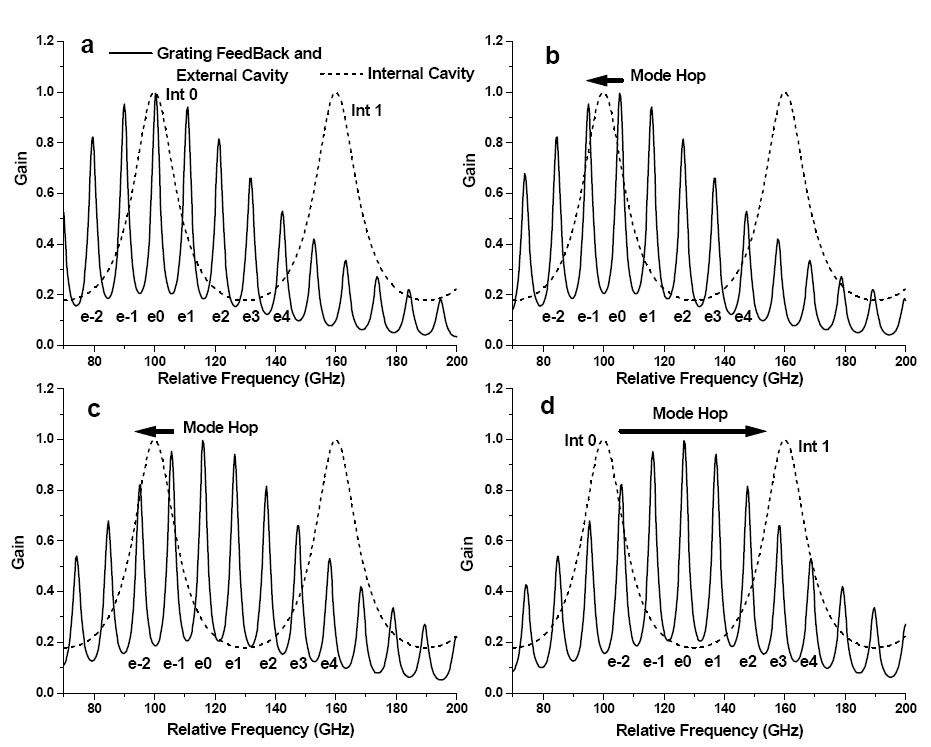
\includegraphics[width=\textwidth]{images/mode_hops.png}
    \caption{Series of graphs showing showing how the external and grating feed back mode shifts
    as the grating angle is changed. \cite{V60}}
    \label{fig:mode_hops}
\end{figure}

While change in the angle will shift the maximum gain of the grating feedback, 
the maximum net gain also depends on the internal cavity gain.
So the emitted frequency will hop from one maximum of the external cavity gain to another maximum. (e.g. e0 to e1 in \autoref{fig:mode_hops})
Eventually the emitted frequency will also hop to another maximum of the internal cavity. (e.g. Int 0 to Int 1 in \autoref{fig:mode_hops})

To prevent these mode hops and allow a continuous sweep through different frequencies, the internal cavity has to be modulated via change in the injection current
simultanously to the change in the grating angle via the piezo crystal.
